\documentclass[11pt,a4paper]{article}

\usepackage{amsfonts,amssymb,amsmath}
\usepackage[margin=1in]{geometry}
\usepackage[none]{hyphenat}
\usepackage{graphicx}
\usepackage{fancyhdr}
\usepackage{float}
\usepackage{color}
\usepackage{xcolor}
\usepackage{tikz}
% Straight quotes in verbatim, so that code copied from the notes runs.
\usepackage{upquote}
\usepackage[nottoc,notlot,notlof]{tocbibind}

\usetikzlibrary{arrows.meta,shapes,positioning}

\parindent 0ex
% hyphenat[none] forbids hyphenation, so give TeX room to stretch a line
% instead of letting it run into the margin.
\setlength{\emergencystretch}{3em}
\setlength{\parskip}{0.55\baselineskip}
\setlength{\abovedisplayskip}{0.5\baselineskip}
\setlength{\belowdisplayskip}{0.5\baselineskip}
\setlength{\abovedisplayshortskip}{0.25\baselineskip}
\setlength{\belowdisplayshortskip}{0.25\baselineskip}
\numberwithin{equation}{section}

\pagestyle{fancy}
\fancyfoot[C]{\thepage}
\fancyhead{}
\fancyhead[R]{\rightmark}
\renewcommand{\headrulewidth}{0pt}

% Upright operator names.
\DeclareMathOperator{\tr}{tr}
\DeclareMathOperator{\rank}{rank}
\DeclareMathOperator{\sgn}{sgn}
\DeclareMathOperator{\Real}{Re}
\DeclareMathOperator{\Imag}{Im}

% Theorem environments.
\usepackage{amsthm}
\theoremstyle{definition}
% One shared counter running section.subsection.n, as in the other courses here.
\newtheorem{thm}{Theorem}[subsection]
\newtheorem{defn}[thm]{Definition}
\newtheorem{exa}[thm]{Example}
\newtheorem{prop}[thm]{Proposition}
\newtheorem{coro}[thm]{Corollary}
\newtheorem{lem}[thm]{Lemma}
% An ``In software'' panel: the R commands, the output they print, and how to read
% it. The web build gives these their own colour (build.py tags the type from
% the label, and ``Software'' is tested before every other label).
\newtheorem{software}[thm]{Software}
\newtheorem*{note}{Note}
\newtheorem*{remark}{Remark}
\newtheorem{problemx}{Problem}[subsection]
\newenvironment{problem}{\begin{problemx}}{\end{problemx}}
\newenvironment{solution}
  {\renewcommand{\qedsymbol}{}\begin{proof}[\textit{Solution}.]}
  {\end{proof}}
\usepackage{enumitem}
% A heading that is legal inside a theorem body, a list or a float, where
% \subsubsection is not. Same weight as \subsubsection* so the two read alike.
\newcommand{\subhead}[1]{%
  \par\medskip\noindent\textbf{#1}\par\nobreak\smallskip}

\begin{document}
% Title page depersonalised for the web, as with every other course here. The
% identity kept below is the Kaplan--Meier estimator, the product of conditional
% survival probabilities on which much of the course is built.
\begin{titlepage}
\thispagestyle{empty}
\begin{center}
\vspace*{3cm}
{\Huge\bfseries Survival Analysis}\\[1.2cm]
{\large Lecture Notes}\\[2.5cm]
\line(1,0){300}\\[1.5cm]
$$\hat S(t) = \prod_{t_j \le t}\Bigl(1 - \frac{d_j}{n_j}\Bigr), \qquad S(t) = \exp\Bigl(-\int_0^t h(u)\,du\Bigr)$$
\end{center}
\end{titlepage}

\tableofcontents
\thispagestyle{empty}
\clearpage
\setcounter{page}{1}

%======================================================================
\section{Survival Data}
\label{sec:data}

Survival analysis is the statistics of \emph{time until something happens}: death after a diagnosis, relapse after treatment, failure of a machine, the end of a spell of unemployment, the default of a loan. Such data look simple, a single positive number for each subject, but they have a feature that ordinary methods cannot handle: for many subjects the event has not
happened by the time the study ends, so their times are only partly known. This section describes survival data, the kinds of incompleteness they have, and why that incompleteness changes the methods we must use.

\subsection{Time-to-event data}
\label{ssec:timetoevent}

A survival study needs three things to be defined clearly:
\begin{itemize}
\item a \textbf{time origin}, the moment from which time is measured: the date of diagnosis, of randomisation in a trial, of installation of a machine, of birth;
\item an \textbf{event}, sometimes called a failure: death, relapse, breakdown, finding a job;
\item a \textbf{time scale}: days, months, years, or another measure such as hours of operation or kilometres driven.
\end{itemize}
The \textbf{survival time} $T$ of a subject is the time from the origin to the event. It is a non-negative random variable, usually with a skewed distribution: many subjects have short times and a few very long ones, so the normal distribution is rarely appropriate.

\begin{exa}
\label{ex:lung}
The \texttt{lung} data in R come from a study of $228$ patients with advanced lung cancer by the North Central Cancer Treatment Group. For each patient we know the number of days from enrolment to death or to the end of follow-up, whether the patient died, and covariates such as age, sex and a performance score measuring how well the patient could
carry out ordinary tasks. Of the $228$ patients, $165$ died during the study and $63$ were still alive when they were last seen (Software~\ref{sw:surv}).
\end{exa}

\subsection{Censoring}
\label{ssec:censoring}

For those $63$ patients the survival time is not known; we know only that it is \emph{longer} than the time at which they were last seen. Such an observation is \textbf{right censored}. It is the most common kind of incompleteness in survival data, and it arises for several reasons:
\begin{itemize}
\item \textbf{the study ends} before the event has happened (administrative censoring);
\item the subject is \textbf{lost to follow-up}: moves away, stops attending;
\item the subject \textbf{withdraws}, or dies of a cause unrelated to the one being studied (if that cause is the event of interest, this is the competing-risks problem of a later section).
\end{itemize}
Three patterns are distinguished. In \textbf{Type I} censoring the study stops at a fixed time, so everyone still alive then is censored at that time. In \textbf{Type II} censoring, used in reliability testing, the study stops when a fixed number of items have failed. Most clinical studies have \textbf{random} censoring: patients enter at different
calendar times and the study ends on one date, so each has a different potential follow-up time (Figure~\ref{fig:followup}).

Other kinds of incompleteness are \textbf{left censoring}, when the event is known only to have happened before some time (a test shows that an infection has already occurred), and \textbf{interval censoring}, when it is known only to have happened between two visits. \textbf{Left truncation}, or delayed entry, is different: subjects enter the study only if they have
survived to some time, so short survivors are never seen at all, as when patients are recruited at a clinic some time after diagnosis.

\begin{figure}[H]
\centering
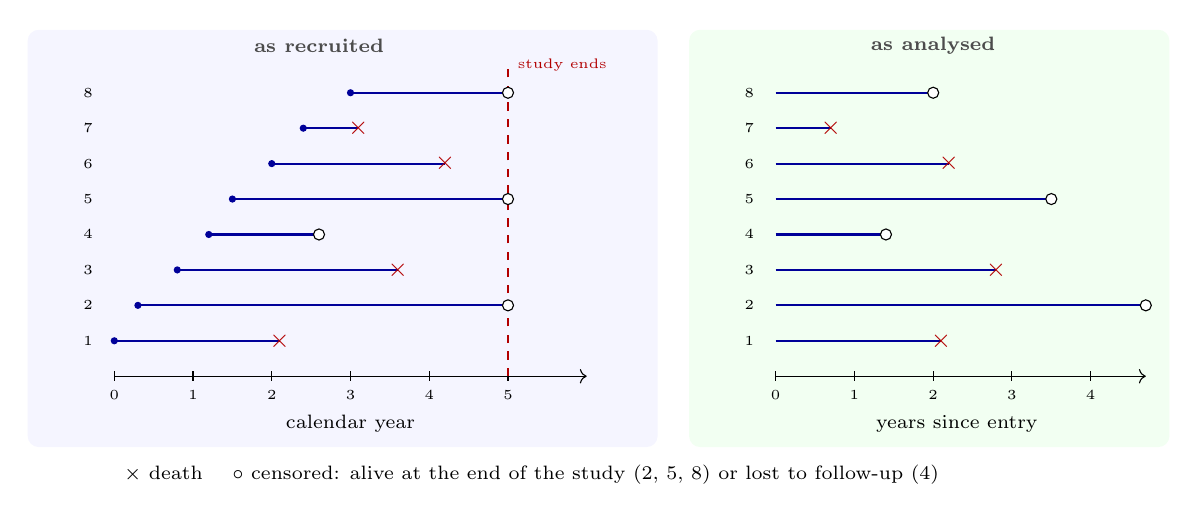
\begin{tikzpicture}[x=1cm,y=1cm]
\begin{scope}
\fill[blue!4,rounded corners=4pt] (-1.1,-0.9) rectangle (6.9,4.4);
\draw[->] (0,0) -- (6.0,0); \node[font=\scriptsize] at (3,-0.6) {calendar year};
\foreach \x in {0,1,...,5} \draw (\x,0.06) -- (\x,-0.06) node[below,font=\tiny] {$\x$};
\draw[red!70!black,dashed] (5,0) -- (5,3.95) node[right,font=\tiny] {study ends};
\foreach \i/\a/\b/\k in {1/0.0/2.1/d, 2/0.3/5.0/c, 3/0.8/3.6/d, 4/1.2/2.6/l, 5/1.5/5.0/c, 6/2.0/4.2/d, 7/2.4/3.1/d, 8/3.0/5.0/c} {
  \node[font=\tiny,anchor=east] at (-0.15,{0.45*\i}) {$\i$};
  \draw[thick,blue!60!black] (\a,{0.45*\i}) -- (\b,{0.45*\i});
  \fill[blue!60!black] (\a,{0.45*\i}) circle (1.3pt);
}
\foreach \i/\b in {1/2.1, 3/3.6, 6/4.2, 7/3.1} \node[red!70!black,font=\small] at (\b,{0.45*\i}) {$\times$};
\foreach \i/\b in {2/5.0, 4/2.6, 5/5.0, 8/5.0} \draw[black,fill=white] (\b,{0.45*\i}) circle (2pt);
\node[font=\scriptsize\bfseries,black!70] at (2.6,4.2) {as recruited};
\end{scope}
\begin{scope}[shift={(8.4,0)}]
\fill[green!5,rounded corners=4pt] (-1.1,-0.9) rectangle (5.0,4.4);
\draw[->] (0,0) -- (4.7,0); \node[font=\scriptsize] at (2.3,-0.6) {years since entry};
\foreach \x in {0,1,...,4} \draw (\x,0.06) -- (\x,-0.06) node[below,font=\tiny] {$\x$};
\foreach \i/\t/\k in {1/2.1/d, 2/4.7/c, 3/2.8/d, 4/1.4/l, 5/3.5/c, 6/2.2/d, 7/0.7/d, 8/2.0/c} {
  \node[font=\tiny,anchor=east] at (-0.15,{0.45*\i}) {$\i$};
  \draw[thick,blue!60!black] (0,{0.45*\i}) -- (\t,{0.45*\i});
}
\foreach \i/\t in {1/2.1, 3/2.8, 6/2.2, 7/0.7} \node[red!70!black,font=\small] at (\t,{0.45*\i}) {$\times$};
\foreach \i/\t in {2/4.7, 4/1.4, 5/3.5, 8/2.0} \draw[black,fill=white] (\t,{0.45*\i}) circle (2pt);
\node[font=\scriptsize\bfseries,black!70] at (2.0,4.2) {as analysed};
\end{scope}
\node[font=\scriptsize,anchor=west] at (0,-1.25) {$\times$ death \quad $\circ$ censored: alive at the end of the study (2, 5, 8) or lost to follow-up (4)};
\end{tikzpicture}
\caption{Eight patients in a study that recruits for three years and ends at year $5$. Left: in calendar time, patients enter at different dates. Right: the same data on the time scale used for analysis, time since entry. Patients $2$, $5$ and $8$ are censored by the end of the study after different lengths of follow-up, and patient $4$ is lost
to follow-up.}
\label{fig:followup}
\end{figure}

\textbf{The key assumption.} Almost every method in this course assumes that censoring is \textbf{non-informative}: a subject censored at time $c$ has the same chance of the event afterwards as subjects still under observation at $c$. Administrative censoring usually satisfies this. Censoring because a patient became too ill to attend does not: those patients are more likely
to die soon, and treating them like the others makes survival look better than it is. The assumption cannot be checked from the data alone, so it must be argued from how the study was run.

\subsection{Why ordinary methods fail}
\label{ssec:whyspecial}

Suppose we want the mean survival time. Two tempting shortcuts are both wrong.
\begin{itemize}
\item Averaging all the recorded times, censored or not, \emph{underestimates} the mean, because censored times are shorter than the true times.
\item Averaging only the uncensored times underestimates it even more, because the subjects who die during the study are disproportionately those with short times; the long survivors are the ones most likely to be censored.
\end{itemize}
In a simulation of $10\,000$ exponential lifetimes with mean $10$, censored at uniform times between $0$ and $20$, the first shortcut gives $5.6$ and the second $4.7$ (Software~\ref{sw:bias}). For exponential data the right estimate of the event rate is the number of events divided by the total time at risk, $\hat\lambda = d/\sum t_i$, and its reciprocal gives
$9.8$; the section on parametric models shows why this is the maximum likelihood estimate. The general lesson is that a censored time carries real information, that the subject survived \emph{at least} that long, and methods must use it rather than discard it or treat it as an event.

\subsection{Recording survival data}
\label{ssec:recording}

Each subject contributes a pair $(t_i, \delta_i)$: the observed time $t_i = \min(T_i, C_i)$, the smaller of the survival time and the censoring time, and the \textbf{event indicator} $\delta_i$, equal to $1$ if the event was observed and $0$ if the time is censored. Covariates are recorded alongside. In R the pair is combined into a \textbf{survival object} with \texttt{Surv(time, event)}, printed with a
\texttt{+} after each censored time. In the \texttt{lung} data the event indicator is coded $2$ for death and $1$ for censored, so \texttt{Surv(time, status == 2)} gives the right object.

Three data sets supplied with R's \texttt{survival} package are used throughout the course: \texttt{lung} (Example~\ref{ex:lung}); \texttt{veteran}, from a Veterans Administration trial of two chemotherapy treatments for lung cancer; and \texttt{ovarian}, a small trial of two treatments for ovarian cancer.

\subsection{Survival data in software}
\label{ssec:software1}

\begin{software}[A survival object]
\label{sw:surv}
The first patients of the \texttt{lung} data, the coding of the status variable, the survival object, and the numbers of events and censored times:
{\small\begin{verbatim}
> library(survival)
> head(lung[, c("time", "status", "age", "sex")], 5)
  time status age sex
1  306      2  74   1
2  455      2  68   1
3 1010      1  56   1
4  210      2  57   1
5  883      2  60   1
> table(lung$status)                    # 1 = censored, 2 = died

  1   2 
 63 165 
> y <- Surv(lung$time, lung$status == 2)
> head(y, 10)                           # a + marks a censored time
 [1]  306   455  1010+  210   883  1022+  310   361   218   166 
> c(events = sum(lung$status == 2), censored = sum(lung$status == 1))
  events censored 
     165       63 
> round(mean(lung$status == 1), 3)      # proportion censored
[1] 0.276
\end{verbatim}}
\textbf{Reading the output.} The third patient was followed for $1010$ days and was still alive, printed $1010+$. There are $165$ deaths and $63$ censored times, so $27.6\%$ of the observations are censored: too many to ignore.

\textbf{Python:} with \texttt{lifelines}, the pair is kept as two columns, \texttt{durations} and \texttt{event\_observed}.
\end{software}

\begin{software}[The cost of ignoring censoring]
\label{sw:bias}
Simulated exponential lifetimes with mean $10$, each censored at an independent uniform time on $(0, 20)$; the fraction of deaths observed, and four estimates of the mean:
{\small\begin{verbatim}
> set.seed(1)
> n <- 10000
> t_true <- rexp(n, rate = 1/10)        # true lifetimes, mean 10
> cens <- runif(n, 0, 20)               # censoring time, uniform on (0, 20)
> time <- pmin(t_true, cens); event <- as.numeric(t_true <= cens)
> round(mean(event), 3)                 # fraction of deaths observed
[1] 0.571
> round(c(true = mean(t_true), all_times = mean(time),
+         deaths_only = mean(time[event == 1]),
+         rate_method = sum(time) / sum(event)), 3)
       true   all_times deaths_only rate_method 
      9.984       5.616       4.674       9.844 
\end{verbatim}}
\textbf{Reading the output.} Only $57\%$ of the deaths are observed. The mean of all recorded times is $5.6$ and the mean of the uncensored times $4.7$, both far below the true mean of about $10$. Dividing the total time at risk by the number of deaths gives $9.84$, close to the truth.

\textbf{Python:} \texttt{numpy.random.exponential} and \texttt{numpy.minimum} give the same simulation.
\end{software}

\begin{software}[Follow-up by group]
\label{sw:followup}
The median recorded time for the deceased and the censored patients in \texttt{lung}, and the numbers and proportions of deaths by sex ($1$ = male, $2$ = female):
{\small\begin{verbatim}
> with(lung, tapply(time, status, median))   # median time by status
  1   2 
284 226 
> with(lung, table(sex, status))
   status
sex   1   2
  1  26 112
  2  37  53
> round(prop.table(with(lung, table(sex, status)), 1), 3)
   status
sex     1     2
  1 0.188 0.812
  2 0.411 0.589
\end{verbatim}}
\textbf{Reading the output.} $81\%$ of the men died during the study but only $59\%$ of the women. This suggests that women survived longer, but the comparison is not yet fair: the groups may have been followed for different lengths of time. The Kaplan--Meier curves and the log-rank test of later sections make such comparisons properly.

\textbf{Python:} \texttt{pandas.crosstab(df.sex, df.status, normalize='index')}.
\end{software}

\subsection{Practice Problems}

\begin{problem}
For each study, state the time origin, the event and the likely causes of censoring: (a) a trial of a drug to prevent a second heart attack; (b) the life of light bulbs tested until $20$ of $50$ have failed; (c) a study of how long graduates take to find their first job.
\end{problem}

\begin{solution}
(a) Origin: randomisation (or the first heart attack); event: a second heart attack; censoring: end of the trial, loss to follow-up, death from other causes (a competing risk). (b) Origin: switching on; event: failure; the $30$ survivors are censored at the time of the $20$th failure, which is Type II censoring. (c) Origin: graduation; event: starting a job;
censoring: end of the survey, emigration, further study (if not counted as the event).
\end{solution}

\begin{problem}
In Figure~\ref{fig:followup}, list the observed pairs $(t_i, \delta_i)$ and give the number of deaths and the total time at risk.
\end{problem}

\begin{solution}
$(2.1, 1)$, $(4.7, 0)$, $(2.8, 1)$, $(1.4, 0)$, $(3.5, 0)$, $(2.2, 1)$, $(0.7, 1)$, $(2.0, 0)$. There are $4$ deaths, and the total time at risk is $2.1 + 4.7 + 2.8 + 1.4 + 3.5 + 2.2 + 0.7 + 2.0 = 19.4$ years, giving an estimated death rate of $4/19.4 = 0.21$ a year if the rate is constant.
\end{solution}

\begin{problem}
A trial records patients as censored when they stop attending because their condition has worsened. Explain how this affects the estimated survival.
\end{problem}

\begin{solution}
The censoring is informative: the patients who leave are at higher risk than those who stay. Methods that assume non-informative censoring treat them as if they had the same future as the remaining patients, so the estimated survival is too high. Where possible, such patients should be traced, or the reason for leaving analysed as an event in its own right.
\end{solution}

\begin{problem}
Distinguish left censoring, interval censoring and left truncation with an example of each.
\end{problem}

\begin{solution}
Left censoring: a child already walks at the first visit, so the age at first walking is only known to be below the age at that visit. Interval censoring: a tumour is absent at one scan and present at the next, so its onset lies between the two dates. Left truncation: a study of the elderly enrols people at age $65$, so anyone who died before $65$ cannot appear, and
each subject's time at risk starts at their age at entry.
\end{solution}

\begin{problem}
Why is the mean of the uncensored times in Software~\ref{sw:bias} even smaller than the mean of all recorded times?
\end{problem}

\begin{solution}
Being uncensored is itself related to the survival time: a subject is uncensored only if $T \leq C$, which is more likely when $T$ is short. Restricting to uncensored subjects therefore selects short survivors. The mean of all recorded times includes the censored subjects at their (too short) censoring times, which are on average longer than the deaths' times, so it is less
biased, though still badly.
\end{solution}

\begin{problem}
A machine-testing laboratory runs $12$ components for $1000$ hours; $5$ fail, at $210$, $430$, $560$, $790$ and $940$ hours, and the rest are still working. What kind of censoring is this, and what is the estimated failure rate per $1000$ hours if it is constant?
\end{problem}

\begin{solution}
Type I censoring at $1000$ hours. The total time at risk is $210 + 430 + 560 + 790 + 940 + 7 \times 1000 = 9930$ hours, so the rate is $5/9930 = 0.000504$ per hour, or $0.50$ per $1000$ hours, and the estimated mean life is $9930/5 = 1986$ hours.
\end{solution}

%SECTIONS

\section*{References}
\addcontentsline{toc}{section}{References}
\sloppy

\subhead{Principal texts}
\begin{enumerate}
\item Collett, D. (2015), \emph{Modelling Survival Data in Medical Research} (3rd ed.), Boca Raton, Chapman \& Hall/CRC.
\item Kleinbaum, D. G., and Klein, M. (2012), \emph{Survival Analysis: A Self-Learning Text} (3rd ed.), New York, Springer.
\item Klein, J. P., and Moeschberger, M. L. (2003), \emph{Survival Analysis: Techniques for Censored and Truncated Data} (2nd ed.), New York, Springer.
\end{enumerate}

\subhead{Recommended texts}
\begin{enumerate}
\item Kalbfleisch, J. D., and Prentice, R. L. (2002), \emph{The Statistical Analysis of Failure Time Data} (2nd ed.), Hoboken, Wiley.
\item Therneau, T. M., and Grambsch, P. M. (2000), \emph{Modeling Survival Data: Extending the Cox Model}, New York, Springer.
\item Hosmer, D. W., Lemeshow, S., and May, S. (2008), \emph{Applied Survival Analysis} (2nd ed.), Hoboken, Wiley.
\end{enumerate}

\subhead{Software}
\begin{enumerate}
\item R Core Team (2024), \emph{R: A Language and Environment for Statistical Computing}, Vienna, R Foundation for Statistical Computing.
\item Therneau, T. M. (2024), \emph{A Package for Survival Analysis in R}, R package \texttt{survival}.
\item Davidson-Pilon, C. (2019), lifelines: survival analysis in Python, \emph{Journal of Open Source Software}, 4(40), 1317.
\end{enumerate}

\subhead{Further reading}
\begin{enumerate}
\item Edmonson, J. H., Fleming, T. R., Decker, D. G., et al. (1979), Different chemotherapeutic sensitivities and host factors affecting prognosis in advanced ovarian carcinoma versus minimal residual disease, \emph{Cancer Treatment Reports}, 63, 241--247.
\item Kaplan, E. L., and Meier, P. (1958), Nonparametric estimation from incomplete observations, \emph{Journal of the American Statistical Association}, 53, 457--481.
\item Leung, K.-M., Elashoff, R. M., and Afifi, A. A. (1997), Censoring issues in survival analysis, \emph{Annual Review of Public Health}, 18, 83--104.
\item Loprinzi, C. L., et al. (1994), Prospective evaluation of prognostic variables from patient-completed questionnaires, \emph{Journal of Clinical Oncology}, 12, 601--607.
\item Prentice, R. L. (1973), Exponential survivals with censoring and explanatory variables, \emph{Biometrika}, 60, 279--288.
\end{enumerate}

\end{document}
